%\documentclass[xcolor=dvipsnames]{beamer}
\documentclass[xcolor=dvipsnames, notes]{beamer}

\usetheme{Warsaw}

\usepackage{inputenc}
\usepackage{amsmath}
\usepackage{amsthm}
\usepackage{graphicx}
%\usepackage{geometry}
\usepackage{tasks}
\ifodd\textwidth
  \addtolength{\textwidth}{1sp}
\fi


\newcommand{\po}{\textcolor{BlueViolet}{po}}
\newcommand{\ppo}{\textcolor{BlueViolet}{ppo}}
\newcommand{\rf}{\textcolor{Green}{rf}}
\newcommand{\rfe}{\textcolor{Green}{rfe}}
\newcommand{\ws}{\textcolor{BurntOrange}{ws}}
\newcommand{\fr}{\textcolor{RubineRed}{fr}}
\newcommand{\com}{\textcolor{BurntOrange}{com}}
\newcommand{\barr}{\textcolor{Apricot}{bar}}

\newcommand{\ghb}{\textcolor{NavyBlue}{ghb}}

\newcommand{\ato}{\textcolor{RoyalPurple}{ato}}


\newcommand{\co}{\textcolor{BurntOrange}{co}}
\newcommand{\mo}{\textcolor{Red}{mo}}
\newcommand{\hbsc}{\textcolor{NavyBlue}{hbsc}}
\newcommand{\xhb}{\textcolor{NavyBlue}{xhb}}
\newcommand{\rfi}{\textcolor{Green}{rfi}}
\newcommand{\brf}{\textcolor{Green}{brf}}
\newcommand{\jhb}{\textcolor{NavyBlue}{jhb}}
\newcommand{\jmo}{\textcolor{Red}{jmo}}

\title{How to Miscompile Programs with Benign Data Races}
\subtitle{Hans. J. Boehm}

\author{Presented by \\ Akshay Gopalakrishnan}

\begin{document}

    \begin{frame}

        \maketitle

    \end{frame}

    \begin{frame}{Introduction}
        
        \begin{itemize}
            \item Programs with Data Races are problematic as their behavior is unpredictable.
            \item Identifying data races are important.
            \item Certain data races are not "harmful" from hardware standpoint, they are "benign" and do not result in program misbehavior. 
            \item However, in languages like C++, such benign races are also harmful due to Compilers.
            \item This paper shows for each category of benign race, how a compiler can optimize code resulting in unpredictable behaviors.
        \end{itemize}

    \end{frame}

    \begin{frame}{Data Race}
        
        \begin{center}
            A data race is when two memory operations accessing the same memory, of which at least one of them is a write, occur simultaneously.
        \end{center}

        \begin{center}
            Two memory operations occur simultaneously if they are next to each other in an interleaved execution order.
        \end{center}

    \end{frame}

    \begin{frame}{Benign Data Race}
        
        \begin{itemize}
            \item Lazy Initialization. 
            \item Reading Old and New values.
            \item Redundant Writes.
            \item Bit Manipulations.
        \end{itemize}
        
    \end{frame}

    \begin{frame}{Reordering across Lazy Initalizations}

        \begin{figure}
            \makebox[\textwidth][c]{
                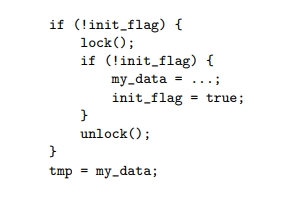
\includegraphics[scale=0.7]{LazyInit.jpeg}
            }
        \end{figure}
        
    \end{frame}

    \note{
        If you want to set the init value to $true$, you can instead do it by double checking the initial value of true.
        This is just to avoid too many writes to the same value of $true$ by multipel threads. 
        It rather helps to read twice, which is much less expensive than one write, which will also trigger cache lines to be invalidated, and so on.
        The proper way to do this however, would be to acquire a global lock, and check once again inside the value of init before changing it. 
        The outer check before lock acquisition will first ensure if the init is updated, do not compete for lock. 
        While the inner check is to save on cycles on repeating writes by different threads.
    }

    \begin{frame}

        \begin{figure}
            \makebox[\textwidth][c]{
                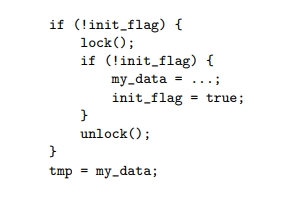
\includegraphics[scale=0.7]{LazyInit.jpeg}
            }
        \end{figure}

    \end{frame}

    \note{
        In the original program, nothing prevents the compiler from reordering the write to data before the write to init flag.
        In a concurrent context, this would violate certain message passing litmus. 
        However, the argument would be that this is done within a lock primitive, so it should be okay.
        But this would be fine only if the reads to both init and data are done only after acquisition of the same lock. 
        Even if this is the case, the compiler can also reordering the read to data above the outer conditional block; thereby changing its value again by introducing a read within the inner conditional block, after data changes.
        This kind of hoisting firstly creates a security problem, wherein temp has the old value of data even if it is not meant to always see it.
    }

    
    \begin{frame}{Introducing Reads to Enable Register Spilling}
        
        \begin{figure}
            \makebox[\textwidth][c]{
                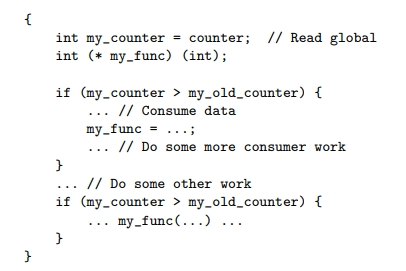
\includegraphics[scale=0.7]{ReadOldVal.jpeg}
            }
        \end{figure}


    \end{frame}

    \note{
        A read write race is bad.
        However, if there is only on write (apart from initialized write), the read-write race can be considered harmless.
        On many occasions, it is in fact okay to simply read either old or new value. 
        On others, it is also okay to read either init or non-init, so in that sense, read-write race is kinda irrelevant and not harmful.
    }

    \begin{frame}
        
        \begin{figure}
            \makebox[\textwidth][c]{
                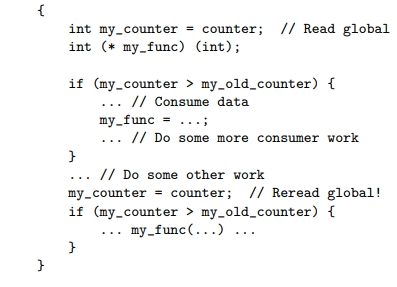
\includegraphics[scale=0.7]{RegisterSpill.jpeg}
            }
        \end{figure}


    \end{frame}

    \note{
        As part of register spilling, which is intended to reuse/optimize use of register memmory, the compiler can introduce a read before the second conditional block.
        This can be done with the assumption that the shared memory value read does not change. 
        And in this case too we have read-write race, where it is considered benign as the read only returns a binary result (either init or non-init).
        But in this program, we could have an additional behavior, one where the conditional expression for both blocks diverge.
    }


    \begin{frame}{Introducing Writes via To Avoid Repeated Writes to Shared Memory}

        \begin{figure}
            \makebox[\textwidth][c]{
                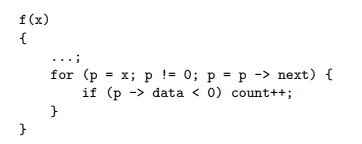
\includegraphics[scale=0.7]{RedundantWrites.jpeg}
            }
        \end{figure}
        
    \end{frame}

    \note{
        Write of the same existing value in memory does not affect the correctness of code. 
        Thus, in this sense redundant write-write data race is harmless.
    }

    \begin{frame}
        \begin{figure}
            \makebox[\textwidth][c]{
                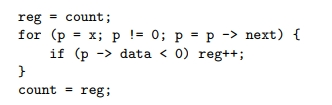
\includegraphics[scale=0.7]{CodeMotionWriteIntro.jpeg}
            }
        \end{figure}

    \end{frame}

    \note{
        As part of Loop code motion, and save cycles on repeated write to shared memory count, the compiler can save the initial value of count into some local register memory. 
        This would introduce a read to count outside the loop.
        The modifications to count within the loop is now modifications to register, which is later written to count after the loop terminates.
        This program, effectively introduces a read and potentially a write to count if the data in $p$ is never negative. 
        Introduction of such reads/writes in a concurrent context leads to security breach (reading the old value of count) as well as violate coherence (write introduction is unsafe).
    }

    \begin{frame}{Reordering Disjoint Bit Manipulations}

        \begin{figure}
            \makebox[\textwidth][c]{
                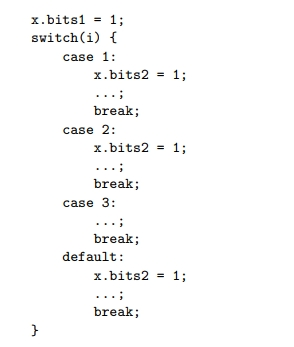
\includegraphics[scale=0.7]{BitManipulation.jpeg}
            }
        \end{figure}
        
    \end{frame}

    \note{
        There can be data races between two memory operations where the programmer knows for sure that the two operations use or modify different bits in a shared variable. 
        Programmers tend to use multiple bits in the same variable in order to optimize for performance.
    }

    \begin{frame}
        \begin{figure}
            \makebox[\textwidth][c]{
                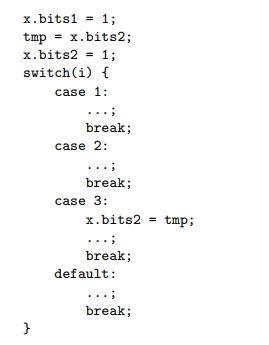
\includegraphics[scale=0.7]{IntroductionWriteBits.jpeg}
            }
        \end{figure}
        
    \end{frame}

    \note{ 
        The compiler can hoist the writes to $x.bits2$ outside the switch, after holding its old value in $tmp$.
        The value is restored if Case 3 is satisfied within the switch.
        This optmization effectively introduces a read and a write to $xbits.2$, if we know the value of $i$ to always be just $3$.
        Thus, in a concurrent context, the bit manipulations on both parts of $x$ would interlave, potentially causing a harmful data race.
    }

    \begin{frame}{Conclusion}

        \begin{itemize}
            \item Benign data races are ideally not meant to cause any programs to misbehave.
            \item However, compilers can optimize code in many ways, making the benign data races to actually cause unpredictable behaviors.
            \item Thus, data races which are harmless from a hardware perspective, is not so in the software stack. 
            \item Correctness of such optimizations must be observed from a concurrent perspective more carefully. 
        \end{itemize}
        
    \end{frame}

\end{document}